\section{Planificación PERT}

\par Con el objetivo de profundizar más en la planificación del proyecto, realizaremos el análisis PERT utilizando el diagrama de red que nos ofrece la herramienta Microsoft Project. En la figura \ref{fig:pert} se ven las relaciones de sucesión entre las tareas, representado en rojo el camino crítico, es decir, aquellas tareas cuyo retraso hará que todo el proyecto se retrase.

%Figura
\begin{figure}[h]
\begin{center}
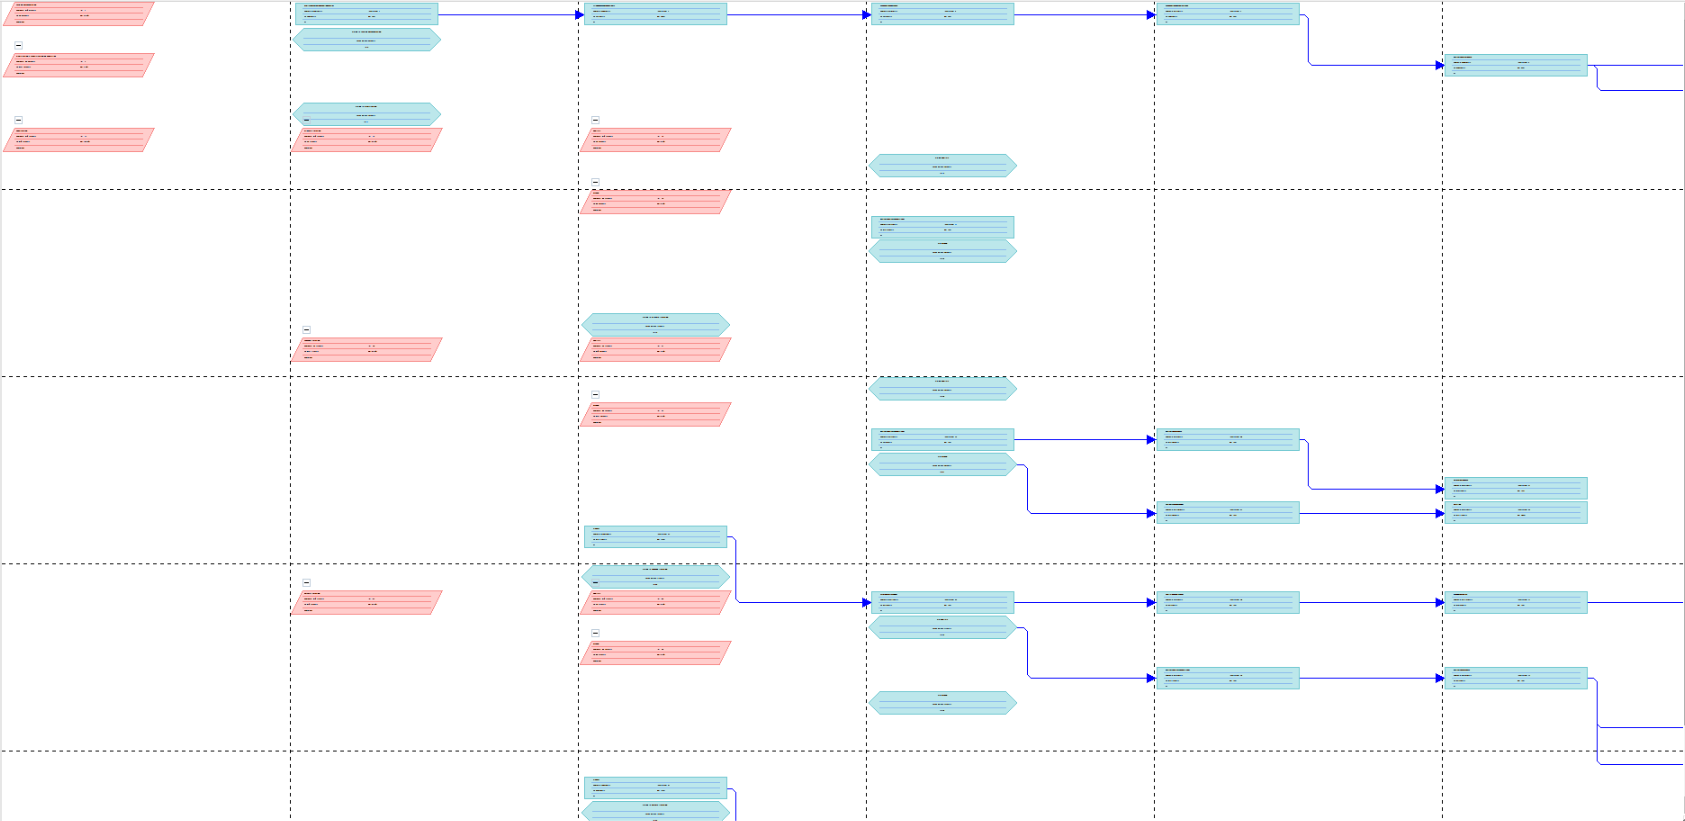
\includegraphics[width=0.6\textwidth]{./img/Pert.png}
\end{center}
\caption{Parte del diagrama PERT}
\label{fig:pert}
\end{figure}

\par Debido a la cantidad de tareas, se muestra únicamente un fragmento del diagrama con el fín de poder explicarlo.

\par Como se puede apreciar en el diagrama, hay algunas tareas, representadas en rojo, cuya finalización es crucial para poder seguir avanzando a tiempo. El conjunto de tareas que forman el camino crítico es el siguiente:

\begin{itemize}[-]
  \item Finalización Fase de Documentación
  \item Finalización Fase Planificación
  \item Modelo Conceptual
  \item Arquitectura del Sistema
  \item Iteración 1
  \begin{itemize}[-]
    \item Refinamiento del plan
    \item Sincronización de modelos
    \item Analisis
    \item Diseño
    \item Desarrollo
    \item Pruebas
  \end{itemize}
  \item Iteración 2
  \begin{itemize}[-]
    \item Refinamiento del plan
    \item Sincronización de modelos
    \item Analisis
    \item Diseño
    \item Desarrollo
    \item Pruebas
  \end{itemize}
  \item Iteración 3
  \begin{itemize}[-]
    \item Refinamiento del plan
    \item Sincronización de modelos
    \item Analisis
    \item Diseño
    \item Desarrollo
    \item Pruebas
  \end{itemize}
  \item Implantación y Fin de Proyecto
\end{itemize}

% \par Por lo tanto esto muestra las tareas que
